% !TeX program = xelatex
\ifdefined\BookMaster\else
\documentclass[11pt,oneside]{article}
% !TeX program = xelatex
\usepackage[b5paper,left=22mm,right=22mm,top=20mm,bottom=22mm,footskip=11mm]{geometry}
\usepackage{fontspec}
\setmainfont{TeX Gyre Termes}
\setsansfont{TeX Gyre Heros}
\usepackage{amsmath,amssymb,mathtools,amsthm}
\renewcommand{\cdots}{\mathinner{\cdotp\cdotp\cdotp}}
\usepackage{graphicx,adjustbox,array,booktabs,longtable,multirow,enumitem,changepage,needspace}
\usepackage[table]{xcolor}
\usepackage{fancyhdr}
\raggedbottom
\interfootnotelinepenalty=10000
\newcommand{\BookFootnote}[2]{\begingroup\renewcommand{\thefootnote}{\fnsymbol{footnote}}\footnote[#1]{#2}\endgroup}
\newcommand{\BookFootnoteMark}[1]{\begingroup\renewcommand{\thefootnote}{\fnsymbol{footnote}}\footnotemark[#1]\endgroup}
\newcommand{\BookFootnoteText}[2]{\begingroup\renewcommand{\thefootnote}{\fnsymbol{footnote}}\footnotetext[#1]{#2}\endgroup}
\newenvironment{BookFloat}[1]{\par\addvspace{.6\baselineskip}\noindent\def\BookFloatID{#1}\begin{minipage}{\linewidth}\phantomsection\label{bookfloat:#1:start}}{\phantomsection\label{bookfloat:\BookFloatID:end}\end{minipage}\par\addvspace{.6\baselineskip}}

\usepackage[unicode,hidelinks]{hyperref}
\pagestyle{fancy}
\fancyhf{}
\newcommand{\BookFooter}{}
\fancyfoot[L]{\parbox[b]{\dimexpr\textwidth-15mm}{\footnotesize\BookFooter}}
\fancyfoot[R]{\footnotesize\thepage}
\renewcommand{\headrulewidth}{0pt}
\renewcommand{\footrulewidth}{0pt}
\setlength{\parindent}{0pt}
\setlength{\parskip}{0.2em}
\setlength{\emergencystretch}{3em}
\setlist{nosep,leftmargin=1.7em,labelsep=.65em}
\newif\ifBookNarrative
\BookNarrativetrue
\newenvironment{BookBody}{\setlength{\parindent}{0pt}}{}
\newcommand{\BookStatement}[1]{\par\addvspace{.6\baselineskip}\noindent #1\enspace\ignorespaces}
\newcommand{\BookLabel}[1]{\par\addvspace{.6\baselineskip}\needspace{3\baselineskip}\noindent\textbf{#1}\quad\ignorespaces}
\newcommand{\BookHeading}[1]{\par\addvspace{\baselineskip}\needspace{4\baselineskip}\noindent{\large\bfseries #1}\par\medskip}
\newcommand{\BookSubheading}[1]{\par\addvspace{.7\baselineskip}\needspace{3\baselineskip}\noindent{\bfseries #1}\par\smallskip}
\newcommand{\BookTextHeading}[1]{\par\addvspace{.7\baselineskip}\needspace{3\baselineskip}\noindent #1\par\smallskip}
\newcommand{\BookSectionTitle}[2]{\par\addvspace{1.2\baselineskip}\needspace{5\baselineskip}\noindent\colorbox{gray!25}{\sffamily\bfseries\small SECTION #1}\quad{\large\bfseries #2}\par\medskip}
\newcommand{\BookExerciseTitle}[1]{\par\addvspace{\baselineskip}\needspace{4\baselineskip}\noindent{\color{gray}\rule{1.5mm}{1.5mm}}\enspace{\large\bfseries Exercises #1}\par\medskip}
\newcommand{\BookBullet}[1]{\begin{list}{\textbullet}{\setlength{\leftmargin}{1.7em}\setlength{\labelwidth}{1em}\setlength{\labelsep}{.7em}\setlength{\topsep}{0pt}\setlength{\parsep}{0pt}\setlength{\itemsep}{0pt}}\item #1\end{list}}
\newcommand{\BookExercise}[2]{\begin{list}{\textbf{#1}}{\setlength{\leftmargin}{2.2em}\setlength{\labelwidth}{1.5em}\setlength{\labelsep}{.7em}\setlength{\topsep}{.15em}\setlength{\parsep}{0pt}\setlength{\itemsep}{0pt}}\item #2\end{list}}
\newcommand{\BookEnd}[1]{\unskip\nobreak\hfill\ensuremath{#1}}
\newcommand{\BookSource}[2]{\phantomsection\label{sourcepage:#1}} % Source-page anchors, retained through reflow.
\usepackage{multicol}
\usepackage{tikz}
\newcommand{\BookPartEntry}[2]{\par\noindent\makebox[17mm][l]{\bfseries Section #1}#2\par}
\newcommand{\BookPartTitle}[3]{\par\bigskip\noindent\begin{tikzpicture}\node[anchor=north west,inner sep=0pt,outer sep=0pt] (bookpart) at (0,0) {\begin{minipage}{\dimexpr\linewidth-.5pt}\hspace*{26mm}\begin{minipage}[t]{\dimexpr\linewidth-26mm}\begin{adjustbox}{max width=\linewidth}{\fontsize{20}{24}\selectfont\bfseries #2}\end{adjustbox}\par\vspace{6mm}\hrule\vspace{6mm}{\sffamily\footnotesize\setlength{\parskip}{.3em}#3}\vspace{3mm}\end{minipage}\end{minipage}};\path[shade,top color=gray!60,bottom color=white] (0,0) rectangle ([xshift=24mm]bookpart.south west);\node[anchor=north,font=\sffamily\bfseries\small] at (12mm,-2mm) {PART};\node[anchor=north,font=\sffamily\bfseries\Huge] at (12mm,-7mm) {#1};\end{tikzpicture}\par\bigskip}
\newsavebox{\BookMathBox}
\makeatletter
\newcommand{\BookInline}[1]{\leavevmode\hskip0pt\relax\begingroup\in@{\begin}{#1}\ifin@\sbox{\BookMathBox}{\(#1\)}\ifdim\wd\BookMathBox>\dimexpr\linewidth-1em\relax\resizebox{\dimexpr\linewidth-1em\relax}{!}{\usebox{\BookMathBox}}\else\(#1\)\fi\else\in@{\left}{#1}\ifin@\sbox{\BookMathBox}{\(#1\)}\ifdim\wd\BookMathBox>\dimexpr\linewidth-1em\relax\resizebox{\dimexpr\linewidth-1em\relax}{!}{\usebox{\BookMathBox}}\else\(#1\)\fi\else\(#1\)\fi\fi\endgroup\hskip0pt\relax}
\makeatother
\DeclareMathOperator{\Aut}{Aut}
\DeclareMathOperator{\End}{End}
\DeclareMathOperator{\Hom}{Hom}
\DeclareMathOperator{\GF}{GF}
\DeclareMathOperator{\irr}{irr}
\DeclareMathOperator{\lt}{lt}
\DeclareMathOperator{\lp}{lp}
\providecommand{\textcircled}[1]{\textnormal{(#1)}}

\begin{document}
\fi
\renewcommand{\BookFooter}{Section 38 Gröbner Bases for Ideals}
\pdfbookmark[0]{Section 38 Gröbner Bases for Ideals}{38_gr_bner_bases_for_ideals}
\ifdefined\BookMaster\else\setcounter{page}{303}\fi
% Source PDF page 320; original printed page 303
\BookSource{320}{303}
\BookNarrativetrue

\begin{BookBody}

\BookSectionTitle{38}{Gröbner Bases for Ideals\label{bookfootnote:320:2:ref}\BookFootnote{2}{\label{bookfootnote:320:2:text}This section is not used in the remainder of the text.}}

\noindent We tackle the problem of finding a nice basis for an ideal \BookInline{I} in \BookInline{F[}\textbf{x}\BookInline{]\; = F[x_{1},\allowbreak x_{2},\allowbreak \cdots,\allowbreak x_{n}].} In view of our Section 37 illustrations for the linear and single indeterminant cases, it seems reasonable to try to replace polynomials in a basis by polynomials of lower degree, or containing fewer indeterminates. It is crucial to have a systematic way to accomplish this. As you probably learned in linear algebra, when row reducing matrices, it is important to follow the standard order for which matrix entries you make zero. If you make an entry in the second column zero before dealing with the first column, you may have wasted your time. As a first step in our goal, we tackle this problem of specifying an order for polynomials in a basis.

\BookTextHeading{\textbf{Ordering Power Products}  }

\noindent Our polynomials in \BookInline{F[}\textbf{x}] have terms of the form \BookInline{ax_{1}^{m_{1}}x_{2}^{m_{2}}\cdots x_{n}^{m_{n}}} where \BookInline{a\in F.} Let us consider a\textbf{ power product} in \BookInline{F[}\textbf{x}] to be an expression

\begin{center}\begin{adjustbox}{max width=\linewidth}\BookInline{\displaystyle P= x_{1}^{m_{1}}x_{2}^{m_{2}}\cdots x_{n}^{m_{n}}\;\text{where all the}\;m_{i}\geq 0\;\text{in}\;\mathbb{Z}.}\end{adjustbox}\end{center}

\noindent Notice that all \BookInline{x_{i}} are present, perhaps some with exponent 0. Thus in \BookInline{F[x,\allowbreak y,\allowbreak z\},\allowbreak } we must write \BookInline{xz^{2}} as \BookInline{xy^{0}z^{2}} to be a power product. We want to describe a\textit{ total ordering} \BookInline{<} on the set of all power products so that we know just what it means to say that \BookInline{P_{i}<P_{j}} for two power products, providing us with a notion of relative size for power products. We can then try to change an ideal basis in a systematic way to create one with polynomials having terms \BookInline{a_{i}P_{i}} with as “small” power products \BookInline{P_{i}} as possible. We denote by 1 the power product with all exponents 0, and require that an ordering of the power products has the properties listed below. Suppose that such an ordering has been described and that \BookInline{P_{i}\neq P_{j}} and \BookInline{P_{i}} divides \BookInline{P_{j}} so that \BookInline{P_{j}= PP_{i}} where \BookInline{1<P.} From Property 4, we then have \BookInline{1P_{i}<PP_{i}= P_{j},\allowbreak } so \BookInline{P_{i}<P_{j}.} Thus \BookInline{P_{i}} divides \BookInline{P_{j}} implies that

\end{BookBody}

% Source PDF page 321; original printed page 304
\BookSource{321}{304}
\BookNarrativetrue

\begin{BookBody}

\noindent \BookInline{P_{i}<P_{j}.} In Exercise 28, we ask you to show by a counterexample that \BookInline{P_{i}<P_{j}} does not imply that \BookInline{P_{i}} divides \BookInline{P_{j}.}

\BookTextHeading{\textbf{Properties for an Ordering of Power Products}  }

\BookExercise{1.}{\BookInline{1<P} for all power products \BookInline{P\neq 1.}}

\BookExercise{2.}{For any two power products \BookInline{P_{i}} and \BookInline{P_{j},\allowbreak } exactly one of \BookInline{P_{i}<P_{j},\allowbreak P_{i}= P_{j},\allowbreak P_{j}<P_{i}} holds.}

\BookExercise{3.}{If \BookInline{P_{i}<P_{j}} and \BookInline{P_{j}<P_{k},\allowbreak } then \BookInline{P_{i}<P_{k}.}}

\BookExercise{4.}{If \BookInline{P_{i}<P_{j},\allowbreak } then \BookInline{PP_{i}<PP_{j}} for any power product \BookInline{P.}}

\noindent It can also be shown that these properties guarantee that any step-by-step process for modifying a finite ideal basis that does not increase the size of any maximal power product in a basis element and replaces at least one by something smaller at each step will terminate in a finite number of steps.

In \BookInline{F[x]} with \BookInline{x} the only indeterminate, there is only one power product ordering, for by Property 1, we must have \BookInline{1<x.} Multiplying repeatedly by \BookInline{x} and using Property 4, we have \BookInline{x<x^{2},\allowbreak x^{2}<x^{3},\allowbreak } etc. Property 3 then shows that \BookInline{1<x<x^{2}<x^{3}<\cdots } is the only possible order. Notice that in Example 37.9, we modified a basis by replacing basis polynomials by polynomials containing smaller power products.

There are a number of possible orderings for power products in \BookInline{F[}\textbf{x}] with \BookInline{n} indeterminates. We present just one, the\textit{ lexicographical order} (denoted by “lex”). In lex, we define

\begin{center}\begin{adjustbox}{max width=\linewidth}\BookInline{\displaystyle x_{1}^{s_{1}}x_{2}^{s_{2}}\cdots x_{n}^{s_{n}}<x_{1}^{t_{1}}x_{2}^{t_{2}}\cdots x_{n}^{t_{n}}(2)}\end{adjustbox}\end{center}

\noindent if and only if \BookInline{s_{i}<t_{i}} for the first subscript \BookInline{i,\allowbreak } reading from left to right, such that \BookInline{s_{i}\neq t_{i}.} Thus in \BookInline{F[x,\allowbreak y],\allowbreak } if we write power products in the order \BookInline{x^{n}y^{m},\allowbreak } we have \BookInline{y= x^{0}y^{1}<} \BookInline{x^{1}y^{0}= x} and \BookInline{xy<xy^{2}.} Using lex, the order of \BookInline{n} indeterminates is given by \BookInline{1<x_{n}<} \BookInline{x_{n- 1}<\cdots <x_{2}<x_{1}.} Our reduction in Example 37.8, where we first got rid of all “big” \BookInline{x}’s that we could and then the “smaller” \BookInline{y}’s, corresponded to the lex order \BookInline{z<y<x,\allowbreak } that is, to writing all power products in the \BookInline{x^{m}y^{n}z^{s}} order. For the two-indeterminate case with \BookInline{y<x,\allowbreak } the total lex term order schematically is

\begin{center}\begin{adjustbox}{max width=\linewidth}\BookInline{\displaystyle 1<y<y^{2}<y^{3}\cdots <x<xy<xy^{2}<xy^{3}<\cdots <x^{2}<x^{2}y<x^{2}y^{2}<\cdots .}\end{adjustbox}\end{center}

\noindent In all the examples that follow we will use lexicographic ordering using a specified ordering of the indeterminates.

An ordering of power products \BookInline{P} induces an obvious ordering of terms\textit{ aP} of a polynomial in \BookInline{F[}\textbf{x}], which we will refer to as a\textbf{ term order.} From now on, given an ordering of power products, we consider every polynomial \BookInline{f} in \BookInline{F[}\textbf{x}] to be written in decreasing order of terms, so that the leading (first) term has the highest order. We denote by 1t\BookInline{(f)} the leading term of \BookInline{f} and by 1p\BookInline{(f)} the power product of the leading term. If \BookInline{f} and \BookInline{g} are polynomials in \BookInline{F[}\textbf{x}] such that 1p\BookInline{(g)} divides 1p\BookInline{(f),\allowbreak } then we can execute a division of \BookInline{f} by \BookInline{g,\allowbreak } as illustrated by the linear and one-indeterminate cases, in Section 37 to obtain \BookInline{f(}\textbf{x}\BookInline{)\; = g(}\textbf{x}\BookInline{)q(}\textbf{x}\BookInline{)\; + r(}\textbf{x}) where 1p\BookInline{(r)<1}p\BookInline{(f).} Note that we did not say that 1p\BookInline{(r)<1}p\BookInline{(g).} We illustrate with an example.

\BookLabel{38.1 Example} By division, reduce the basis \BookInline{\{xy^{2},\allowbreak y^{2}- y\}} for the ideal \BookInline{I= \langle xy^{2},\allowbreak y^{2}- y\rangle } in \BookInline{\mathbb{R}[x,\allowbreak y]} to one with smaller maximum term size, assuming the order lex with \BookInline{y<x.}

\end{BookBody}

% Source PDF page 322; original printed page 305
\BookSource{322}{305}
\BookNarrativetrue

\begin{BookBody}

\BookLabel{\textit{Solution}} We see that \BookInline{y^{2}} divides \BookInline{xy^{2}} and compute

\begin{center}\begin{adjustbox}{max width=\linewidth}\BookInline{\displaystyle \begin{aligned}&x \\ &y^{2}- yxy^{2} \\ &xy^{2}- xy \\ &xy\end{aligned}}\end{adjustbox}\end{center}

\noindent Because \BookInline{y^{2}} does not divide \BookInline{xy,\allowbreak } we cannot continue the division. Note that 1p\BookInline{(xy)= xy} is not less than 1p\BookInline{(y^{2}- y)= y^{2}.} However, we do have 1p\BookInline{(xy)<1}p\BookInline{(xy^{2}).} Our new basis for \BookInline{I} is \BookInline{\{xy,\allowbreak y^{2}- y\}.}\BookEnd{\blacktriangle}

When dealing with more than one indeterminate, it is often easier to perform basis reduction by multiplying a basis polynomial \BookInline{g(}\textbf{x}) by a polynomial \BookInline{- q(}\textbf{x}) and adding it to a polynomial \BookInline{f(}\textbf{x}) to obtain \BookInline{r(}\textbf{x}), as we perform matrix reduction in linear algebra, rather than writing out the division display as we did in the preceding example. Starting with basis polynomials \BookInline{xy^{2}} and \BookInline{y^{2}- y,\allowbreak } we can reduce the \BookInline{xy^{2}} by multiplying \BookInline{y^{2}- y} by \BookInline{- x} and adding the resulting \BookInline{- xy^{2}+ xy} to \BookInline{xy^{2},\allowbreak } obtaining the replacement \BookInline{xy} for \BookInline{xy^{2}.} We can do that in our head, and write down the result directly.

Referring again to Example 38.1, it will follow from what we state later that given any polynomial \BookInline{f(x,\allowbreak y)= c_{1}(x,\allowbreak y)(xy)+ c_{2}(x,\allowbreak y)(y^{2}- y)} in \BookInline{\langle xy,\allowbreak y^{2}- y\rangle,\allowbreak } either \BookInline{xy} or \BookInline{y^{2}} will divide 1p\BookInline{(f).(}See Exercise 32.) This illustrates the defining property of a \BookInline{Gro}\textit{¨}\BookInline{bner} \textit{basis}.

\BookLabel{38.2 Definition} A set \BookInline{\{g_{1},\allowbreak g_{2},\allowbreak \cdots,\allowbreak g_{r}\}} of nonzero polynomials in \BookInline{F[x_{1},\allowbreak x_{2},\allowbreak \cdots,\allowbreak x_{n}],\allowbreak } with term ordering \BookInline{<,\allowbreak } is a\textbf{ Gröbner basis} for the ideal \BookInline{I= \langle g_{1},\allowbreak g_{2},\allowbreak \cdots,\allowbreak g_{r}\rangle } if and only if, for each nonzero \BookInline{f\in I,\allowbreak } there exists some \BookInline{i} where \BookInline{1\leq i\leq r} such that 1p\BookInline{(g_{i})} divides 1p\BookInline{(f).}\BookEnd{\blacksquare}

While we have illustrated the computation of a Gröbner basis from a given basis for an ideal in Examples 37.8, 37.9, and 38.1, we have not given a specific algorithm. We refer the reader to Adams and Loustaunau [23]. The method consists of multiplying some polynomial in the basis by any polynomial in \BookInline{F[}\textbf{x}] and adding the result to another polynomial in the basis in a manner that reduces the size of power products. In our illustrations, we have treated the case involving division of \BookInline{f(}\textbf{x}) by \BookInline{g(}\textbf{x}) where 1p\BookInline{(g)} divides 1p\BookInline{(f),\allowbreak } but we can also use the process if 1p\BookInline{(g)} only divides some other power product in \BookInline{f.} For example, if two elements in a basis are \BookInline{xy- y^{3}} and \BookInline{y^{2}- 1,\allowbreak } we can multiply \BookInline{y^{2}- 1} by \BookInline{y} and add it to \BookInline{xy- y^{3},\allowbreak } reducing \BookInline{xy- y^{3}} to \BookInline{xy- y.} Theorem 37.7 shows that this is a valid computation.

You may wonder how any basis \BookInline{\{g_{1},\allowbreak g_{2},\allowbreak \cdots,\allowbreak g_{r}\}} can fail to be a Gröbner basis for \BookInline{I= \langle g_{1},\allowbreak g_{2},\allowbreak \cdots,\allowbreak g_{r}\rangle } because, when we form an element \BookInline{c_{1}g_{1}+ c_{2}g_{2}+ \cdots + c_{r}g_{r}} in \BookInline{I,\allowbreak } we see that 1p\BookInline{(g_{i})} is a divisor of 1p\BookInline{(c_{i}g_{i})} for \BookInline{i= 1,\allowbreak 2,\allowbreak \cdots,\allowbreak r.} However, cancellation of power products can occur in the addition. We illustrate with an example.

\BookLabel{38.3 Example} Consider the ideal \BookInline{I= \langle x^{2}y- 2,\allowbreak xy^{2}- y\rangle } in \BookInline{\mathbb{R}[x,\allowbreak y\}.} The polynomials in the basis shown cannot be reduced further. However, the ideal \BookInline{I} contains \BookInline{y(x^{2}y- 2)- x(xy^{2}- y)= xy- } \BookInline{2y,\allowbreak } whose leading power product \BookInline{xy} is not divisible by either of the leading power products \BookInline{x^{2}y} or \BookInline{xy^{2}} of the given basis. Thus \BookInline{\{x^{2}y- 2,\allowbreak xy^{2}- y\}} is not a Gröbner basis for \BookInline{I,\allowbreak } according to Definition \BookInline{38.2.}\BookEnd{\blacktriangle}

When we run into a situation like that in Example 38.3, we realize that a Gröbner basis must contain some polynomial with a smaller leading power product than those in the given basis. Let \BookInline{f} and \BookInline{g} be polynomials in the given basis. Just as we did in Example 38.3, we can multiply \BookInline{f} and \BookInline{g} by as small power products as possible so that the resulting two leading power products will be the same, the\textit{ least common multiple}

\end{BookBody}

% Source PDF page 323; original printed page 306
\BookSource{323}{306}
\BookNarrativetrue

\begin{BookBody}

\noindent (lcm) of 1p\BookInline{(f)} and 1p\BookInline{(g),\allowbreak } and then subtract or add with suitable coefficients from \BookInline{F} so cancellation results. We denote a polynomial formed in this fashion by \BookInline{S(f,\allowbreak g).} We state without proof a theorem that can be used to test whether a basis is a Gröbner basis.

\BookLabel{38.4 Theorem} A basis \BookInline{G= \{g_{1},\allowbreak g_{2},\allowbreak \cdots,\allowbreak g_{r}\}} is a Gröbner basis for the ideal \BookInline{\langle g_{1},\allowbreak g_{2},\allowbreak \cdots,\allowbreak g_{r}\rangle } if and only if, for all \BookInline{i\neq j,\allowbreak } the polynomial \BookInline{S(g_{i},\allowbreak g_{j})} can be reduced to zero by repeatedly dividing remainders by elements of \BookInline{G,\allowbreak } as in the division algorithm.

As we mentioned before, we may prefer to think of reducing \BookInline{S(g_{i},\allowbreak g_{j})} by a sequence of operations consisting of adding (or subtracting) multiples of polynomials in \BookInline{G,\allowbreak } rather than writing out division.

We can now indicate how we can obtain a Gröbner basis from a given basis. First, reduce the polynomials in the basis as far as possible among themselves. Then choose polynomials \BookInline{g_{i}} and \BookInline{g_{j}} in the basis, and form the polynomial \BookInline{S(g_{i},\allowbreak g_{j}).} See if \BookInline{S(g_{i},\allowbreak g_{j})} can be reduced to zero as just described. If so, choose a different pair of polynomials, and repeat the procedure with them. If \BookInline{S(g_{i},\allowbreak g_{j})} cannot be reduced to zero as described above, augment the given basis with this \BookInline{S(g_{i},\allowbreak g_{j}),\allowbreak } and start all over, reducing this basis as much as possible. By Theorem 38.4, when every polynomial \BookInline{S(g_{i},\allowbreak g_{j})} for all \BookInline{i\neq j} can be reduced to zero using polynomials from the latest basis, we have arrived at a Gröbner basis. We conclude with a continuation of Example 38.3.

\BookLabel{38.5 Example} Continuing Example 38.3, let \BookInline{g_{1}= x^{2}y- 2,\allowbreak g_{2}= xy^{2}- y,\allowbreak } and \BookInline{I= \langle g_{1},\allowbreak g_{2}\rangle } in \BookInline{\mathbb{R}^{2}.} In Example 38.3, we obtained the polynomial \BookInline{S(g_{1},\allowbreak g_{2})= xy- 2y,\allowbreak } which cannot be reduced to zero using \BookInline{g_{1}} and \BookInline{g_{2}.} We now reduce the basis \BookInline{\{x^{2}y- 2,\allowbreak xy^{2}- y,\allowbreak xy- 2y\},\allowbreak } indicating each step.

\begin{center}\begin{adjustbox}{max width=\linewidth}\BookInline{\displaystyle \{x^{2}y- 2,\allowbreak xy^{2}- y,\allowbreak xy- 2y\}\;\text{augmented basis}\;}\end{adjustbox}\end{center}

\begin{center}\begin{adjustbox}{max width=\linewidth}\BookInline{\displaystyle \{2xy- 2,\allowbreak xy^{2}- y,\allowbreak xy- 2y\}\;\text{by adding}\;(- x)(\;\text{third}\;)\;\text{to}\;\text{fi}\;\text{rst}\;}\end{adjustbox}\end{center}

\begin{center}\begin{adjustbox}{max width=\linewidth}\BookInline{\displaystyle \{2xy- 2,\allowbreak 2y^{2}- y,\allowbreak xy- 2y\}\;\text{by adding}\;(- y)(\;\text{third}\;)\;\text{to second}\;}\end{adjustbox}\end{center}

\begin{center}\begin{adjustbox}{max width=\linewidth}\BookInline{\displaystyle \{4y- 2,\allowbreak 2y^{2}- y,\allowbreak xy- 2y\}\;\text{by adding}\;(- 2)(\;\text{third}\;)\;\text{to}\;\text{fi}\;\text{rst}\;}\end{adjustbox}\end{center}

\begin{center}\begin{adjustbox}{max width=\linewidth}\BookInline{\displaystyle \{4y- 2,\allowbreak 0,\allowbreak xy- 2y\}\;\text{by adding}\;(- \frac{y}{2})(\text{fi}\;\text{rst}\;)\;\text{to second}\;}\end{adjustbox}\end{center}

\begin{center}\begin{adjustbox}{max width=\linewidth}\BookInline{\displaystyle \{4y- 2,\allowbreak 0,\allowbreak \frac{1}{2}x- 2y\}\;\text{by adding}\;(- \frac{x}{4})(\text{fi}\;\text{rst}\;)\;\text{to third}\;}\end{adjustbox}\end{center}

\begin{center}\begin{adjustbox}{max width=\linewidth}\BookInline{\displaystyle \{4y- 2,\allowbreak 0,\allowbreak \frac{1}{2}x- 1\}\;\text{by adding}\;(\frac{1}{2})(\text{fi}\;\text{rst}\;)\;\text{to third}\;}\end{adjustbox}\end{center}

\noindent Clearly\BookInline{,\allowbreak \{y- \frac{1}{2},\allowbreak x- 2\}} is a Gröbner basis. Note that if \BookInline{f= y- \frac{1}{2}} and \BookInline{g= x- 2,\allowbreak } then \BookInline{S(f,\allowbreak g)= xf- yg= (xy- \frac{x}{2})- (xy- 2y)= - \frac{x}{2}+ 2y,\allowbreak } which can readily be reduced to zero by adding \BookInline{\textstyle { \frac { 1 } { 2 } } ( x - 2 )} and \BookInline{- 2(y- \frac{1}{2}).}

From the Gröbner basis, we see that the algebraic variety \BookInline{V(I)} contains only one point, (2, 12 ), in \BookInline{\mathbb{R}^{2}.}\BookEnd{\blacktriangle}

\BookTextHeading{\textbf{Applications}}

\noindent Here we give a simple example of how a Gröbner basis can be used to derive a geometric formula.

\BookLabel{38.6 Example} Using a Gröbner basis, derive the standard formula for a parabola.

\BookLabel{\textit{Solution}} Recall that a parabola is the set of all points in the plane that are equidistant from a fixed line (directrix) and a fixed point (focus). In standard form, the directrix is the line \BookInline{y= - p} and the focus is the point \BookInline{(0,\allowbreak p)} where \BookInline{p>0.} The algebraic variety defined by the ideal \BookInline{\langle x^{2}+ (y- p)^{2}- d^{2},\allowbreak y+ p- d\rangle } gives the set of all points \BookInline{(x_{0},\allowbreak y_{0},\allowbreak p_{0},\allowbreak d_{0})\in \mathbb{R}^{4}} 
% Source PDF page 324; original printed page 307
\BookSource{324}{307}
such that the point \BookInline{(x_{0},\allowbreak y_{0})} is a distance of \BookInline{d_{0}} from the point \BookInline{(0,\allowbreak p_{0})} and a distance \BookInline{d_{0}} from the line \BookInline{y= - p.} We order the indeterminates by \BookInline{p<x<y<d} and seek a Gröbner basis.

\end{BookBody}

\BookNarrativetrue

\begin{BookBody}

\begin{center}\begin{adjustbox}{max width=\linewidth}\BookInline{\displaystyle \begin{aligned}&\{- d^{2}+ y^{2}- 2yp+ x^{2}+ p^{2},\allowbreak d- y- p\}\;\text{initial basis}\; \\ &\{- dy- dp+ y^{2}- 2yp+ x^{2}+ p^{2},\allowbreak d- y- p\}\;\text{by adding}\;(\mathrm{d})(\;\text{second}\;)\;\text{to}\;\text{fi}\;\text{rst}\; \\ &\{- dp- 3yp+ x^{2}+ p^{2},\allowbreak d- y- p\}\;\text{by adding}\;(\mathrm{y})(\;\text{second}\;)\;\text{to}\;\text{fi}\;\text{rst}\; \\ &\{- 4yp+ x^{2},\allowbreak d- y- p\}\;\text{by adding}\;(\mathrm{p})(\;\text{second}\;)\;\text{to}\;\text{fi}\;\text{rst}\;\end{aligned}}\end{adjustbox}\end{center}

In Exercise 33 you are asked to check that \BookInline{\{- 4yp+ x^{2},\allowbreak d- y- p\}} is a Gröbner basis. Note that for any \BookInline{(x_{0},\allowbreak y_{0},\allowbreak p_{0})\in \mathbb{R}^{3}} that is a zero of the first polynomial \BookInline{- 4yp+ x^{2},\allowbreak } there is a real number \BookInline{d_{0}} so that \BookInline{(x_{0},\allowbreak y_{0},\allowbreak p_{0},\allowbreak d_{0})} is a zero of the second polynomial. This verifies the standard form of the equation of a parabola\BookInline{,\allowbreak 4py= x^{2}.}\BookEnd{\blacktriangle}

\begin{BookFloat}{38_gr_bner_bases_for_ideals-p324-3}
\begin{center}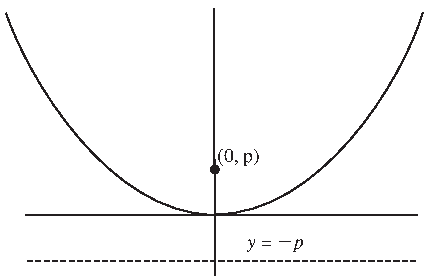
\includegraphics[width=0.586\linewidth,height=.8\textheight,keepaspectratio]{assets/p324_04.pdf}\end{center}
\end{BookFloat}

Care must be taken in deciding the order for the indeterminate. In Example 38.6, had we taken the order of the indeterminates to be \BookInline{d<p<x<y,\allowbreak } the resulting Gröbner basis would have been \BookInline{\{- 4dp+ 4p^{2}+ x^{2},\allowbreak d- p- y\},\allowbreak } which does not directly give the standard form for the equation of a parabola. The reason for making the indeterminate \BookInline{d} the largest is that the algorithm attempts to eliminate \BookInline{d} from polynomials in the basis since the reduction process reduces the maximum-sized term.

The algorithm for computing Gröbner bases can be programmed. In fact, it is a built-in function on many common mathematical packages including Mathematica, Maple, Wolfram Alpha, and others. By carefully picking the order of the indeterminates, it is possible to solve a large variety of problems using automated computations of Gröbner bases.

\BookLabel{38.7 Example} We use a software package to compute a Gröbner basis that yields the equation of an ellipse in standard position. An ellipse in standard position is the set of all points in the plane so that the sum of the distances to the two foci \BookInline{(c,\allowbreak 0)} and \BookInline{(- c,\allowbreak 0)} is a fixed distance \BookInline{2a.} We start with the basis

\begin{center}\begin{adjustbox}{max width=\linewidth}\BookInline{\displaystyle \{(x- c)^{2}+ y^{2}- d_{1}^{2},\allowbreak (x+ c)^{2}+ y^{2}- d_{2}^{2},\allowbreak d_{1}+ d_{2}- 2a\}}\end{adjustbox}\end{center}

\noindent where \BookInline{d_{1}} represents the distance to focus \BookInline{(c,\allowbreak 0)} and \BookInline{d_{2}} represents the distance to focus \BookInline{(- c,\allowbreak 0).} We wish to arrive at a polynomial that includes \BookInline{x} and \BookInline{y} as well as the parameters \BookInline{a} and \BookInline{c} that describe the shape and size of the ellipse. Therefore, we take \BookInline{d_{1}} and \BookInline{d_{2}} as the largest indeterminates. Using the order \BookInline{a<c<y<x<d_{2}<d_{1},\allowbreak } a mathematical software package quickly computes the Gröbner basis

\begin{center}\begin{adjustbox}{max width=\linewidth}\BookInline{\displaystyle \{a^{4}- a^{2}c^{2}- a^{2}x^{2}+ c^{2}x^{2}- a^{2}y^{2},\allowbreak - a^{2}+ ad_{2}- cx,\allowbreak a^{3}- ac^{2}- acs+ cd_{2}x- ax^{2}- ay^{2},\allowbreak }\end{adjustbox}\end{center}

\begin{center}\begin{adjustbox}{max width=\linewidth}\BookInline{\displaystyle - c^{2}+ d_{2}^{2}- 2cx- x^{2}- y^{2},\allowbreak - 2a+ d_{1}+ d_{2}\}.}\end{adjustbox}\end{center}

\end{BookBody}

% Source PDF page 325; original printed page 308
\BookSource{325}{308}
\BookNarrativetrue

\begin{BookBody}

\noindent The first polynomial can be written as

\begin{center}\begin{adjustbox}{max width=\linewidth}\BookInline{\displaystyle a^{2}(a^{2}- c^{2})- (a^{2}- c^{2})x^{2}- a^{2}y^{2}.}\end{adjustbox}\end{center}

\noindent We think of \BookInline{a} and \BookInline{c} as parameters and recall that in an ellipse, the parameter \BookInline{b>0} is defined by \BookInline{b^{2}= a^{2}- c^{2}.} We see that the variety in \BookInline{\mathbb{R}^{2}} defined from the ideal \BookInline{\langle a^{2}b^{2}- } \BookInline{b^{2}x^{2}- a^{2}y^{2}\rangle } has equation

\begin{center}\begin{adjustbox}{max width=\linewidth}\BookInline{\displaystyle { \frac { x ^ { 2 } } { a ^ { 2 } } } + { \frac { y ^ { 2 } } { b ^ { 2 } } } = 1 .}\end{adjustbox}\end{center} \BookEnd{\blacktriangle}

A\textbf{ graph} is a finite set with elements called\textbf{ vertices} together with a collection of pairs of vertices called\textbf{ edges} or\textbf{ arcs}. Graphs are often drawn as in Figure 38.10, which shows a graph with four vertices \BookInline{x_{1},\allowbreak x_{2},\allowbreak x_{3},\allowbreak x_{4}} and four edges \BookInline{\{x_{1},\allowbreak x_{2}\},\allowbreak \{x_{2},\allowbreak x_{3}\},\allowbreak \{x_{3},\allowbreak x_{1}\},\allowbreak } \BookInline{\{x_{3},\allowbreak x_{4}\}.} A\textbf{ coloring} of a graph is an assignment of colors to the vertices in such a way that no two vertices in the same edge have the same color. The problem of determining if a graph can be colored with \BookInline{n} colors can be restated as a question about an ideal, which can (at least theoretically) be answered using Gröbner bases.

\BookLabel{38.8 Theorem} Let \BookInline{G} be a graph with vertex set \BookInline{\{x_{1},\allowbreak x_{2},\allowbreak...,\allowbreak x_{k}\}.} We identify each vertex with an indeterminate and form the ideal \BookInline{I\subseteq \mathbb{C}[x_{1},\allowbreak x_{2},\allowbreak...,\allowbreak x_{k}]} with basis consisting of polynomials \BookInline{x_{1}- 1,\allowbreak x_{2}^{n}- 1,\allowbreak x_{3}^{n}- 1,\allowbreak...,\allowbreak x_{k}^{n}- 1} together with a polynomial \BookInline{x}\textit{in}\BookInline{- 1+ x}\textit{in}\BookInline{- 2xj+ x}\textit{in}\BookInline{- 3xj2+ } \BookInline{\cdots + x_{i}x_{j}^{n- 2}+ x_{j}^{n- 1}} for each edge in the graph. The graph \BookInline{G} can be colored with \BookInline{n} colors if and only if the algebraic variety \BookInline{V(I)} is nonempty.

\BookLabel{\textit{Proof}} The proof is left for Exercise 34. \BookEnd{\blacklozenge}

The variety \BookInline{V(I)} in Theorem 38.8 gives all possible colorings of the graph \BookInline{G} using the \BookInline{n ^ { \mathrm { t h } }} roots of unity for the colors and coloring vertex \BookInline{x_{1}} with the color 1. For each point in \BookInline{V(I),\allowbreak } the \BookInline{j ^ { \mathrm { t h } }} coordinate gives the color assigned to \BookInline{x_{j}.}

\BookLabel{38.9 Example} Using the graph in Figure 38.10, the basis described in Theorem 38.8 for \BookInline{n= 2} is

\begin{center}\begin{adjustbox}{max width=\linewidth}\BookInline{\displaystyle \{x_{1}- 1,\allowbreak x_{2}^{2}- 1,\allowbreak x_{3}^{2}- 1,\allowbreak x_{4}^{2}- 1,\allowbreak x_{1}+ x_{2},\allowbreak x_{2}+ x_{3},\allowbreak x_{3}+ x_{1},\allowbreak x_{3}+ x_{4}\}.}\end{adjustbox}\end{center}

\noindent A Gröbner basis is \BookInline{\{1\}.} This can be determined electronically, or by noticing that

\begin{center}\begin{adjustbox}{max width=\linewidth}\BookInline{\displaystyle (x_{1}+ x_{2})- (x_{2}+ x_{3})+ (x_{3}+ x_{1})= 2x_{1}\in I.}\end{adjustbox}\end{center}

\noindent Therefore\BookInline{,\allowbreak x_{1}\in I,\allowbreak } so \BookInline{x_{1}- (x_{1}- 1)= 1\in I.} Thus the ideal is all of \BookInline{\mathbb{C}[x_{1},\allowbreak x_{2},\allowbreak x_{3},\allowbreak x_{4}],\allowbreak } which has \BookInline{\{1\}} as a basis. Since the algebraic variety for \BookInline{\langle 1\rangle } is the empty set, the graph cannot be colored with two colors.

We now compute a Gröbner basis when \BookInline{n= 3.} Theorem 38.8 tells us to start with the basis

\begin{BookFloat}{38_gr_bner_bases_for_ideals-p325-16}
\begin{center}\small \textbf{38.10 Figure}\end{center}
\begin{center}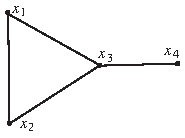
\includegraphics[width=0.254\linewidth,height=.8\textheight,keepaspectratio]{assets/review_v3_p325_38.10.pdf}\end{center}
\end{BookFloat}

\begin{center}\begin{adjustbox}{max width=\linewidth}\BookInline{\displaystyle \begin{aligned}&\{x_{1}- 1,\allowbreak x_{2}^{3}- 1,\allowbreak x_{3}^{3}- 1,\allowbreak x_{4}^{3}- 1,\allowbreak x_{1}^{2}+ x_{1}x_{2}+ x_{2}^{2},\allowbreak x_{2}^{2}+ x_{2}x_{3}+ x_{3}^{2},\allowbreak x_{3}^{2}+ x_{3}x_{1} \\ &+ x_{1}^{2},\allowbreak x_{3}^{2}+ x_{3}x_{4}+ x_{4}^{2}\}.\end{aligned}}\end{adjustbox}\end{center}

\noindent Using a software package, a Gröbner basis with indeterminate order \BookInline{x_{1}<x_{2}<x_{3}<x_{4}} is

\begin{center}\begin{adjustbox}{max width=\linewidth}\BookInline{\displaystyle \{x_{1}- 1,\allowbreak x_{2}^{2}+ x_{2}+ 1,\allowbreak 1+ x_{2}+ x_{3},\allowbreak x_{2}- x_{4}- x_{2}x_{4}+ x_{4}^{2}\}.}\end{adjustbox}\end{center}

\noindent Let $\zeta=-\frac{\sqrt{3}}{2}+\frac{1}{2}i$ be a third root of unity. We find an element $(a_1,a_2,a_3,a_4)\in V(I)$:
% The printed source has -sqrt(3)/2 + i/2 here. This is retained faithfully;
% it is a source erratum (a cube root would instead be -1/2 + sqrt(3)i/2).
\[
\begin{aligned}
a_1-1 &= 0 && a_1=1,\\
a_2^2+a_2+1 &= 0 && \begin{aligned}[t]
 &\text{$a_2$ is a third root of unity.}\\
 &\text{Let }a_2=\zeta.
 \end{aligned}\\
1+\zeta+a_3 &= 0 && a_3=-1-\zeta=\zeta^2,\\
\zeta-a_4-\zeta a_4+a_4^2 &= 0 && \begin{aligned}[t]
 &\text{factoring,}\\
 &(\zeta-a_4)(1-a_4)=0.
 \end{aligned}
\end{aligned}
\]

\end{BookBody}

% Source PDF page 326; original printed page 309
\BookSource{326}{309}
\BookNarrativetrue

\begin{BookBody}

\noindent We see that we can color vertex 1 the color 1, vertex \BookInline{2\zeta,\allowbreak } vertex \BookInline{3\zeta ^{2},\allowbreak } and then we can color vertex 4 either the color 1 or \BookInline{\zeta.}\BookEnd{\blacktriangle}

There are many applications of Gröbner bases in mathematics, statistics, engineering, and computer science. These include controlling robot arms and automated theorem proving. The algorithm to compute a Gröbner basis is generally too long and tedious to be done by hand, so computers are essential. However, some larger problems are not feasible even on modern high-speed computers.

\end{BookBody}

\BookNarrativefalse

\begin{BookBody}

\BookExerciseTitle{38}

\noindent In Exercises 1 through 4, write the polynomials in \BookInline{\mathbb{R}[x,\allowbreak y,\allowbreak z]} in decreasing term order, using the order lex for power products \BookInline{x^{m}y^{n}z^{s}} where \BookInline{z<y<x.}

\BookExercise{1.}{\BookInline{2xy^{3}z^{5}- 5x^{2}yz^{3}+ 7x^{2}y^{2}z- 3x^{3}}}

\BookExercise{2.}{\BookInline{3y^{2}z^{5}- 4x+ 5y^{3}z^{3}- 8z^{7}}}

\BookExercise{3.}{\BookInline{3y- 7x+ 10z^{3}- 2xy^{2}z^{2}+ 2x^{2}yz^{2}}}

\BookExercise{4.}{\BookInline{38- 4xz+ 2yz- 8xy+ 3yz^{3}}}

\noindent In Exercises 5 through 8, write the polynomials in \BookInline{\mathbb{R}[x,\allowbreak y,\allowbreak z]} in decreasing term order, using the order lex for power products \BookInline{z^{m}y^{n}x^{s}} where \BookInline{x<y<z.}

\BookExercise{5.}{The polynomial in Exercise 1.}

\BookExercise{6.}{The polynomial in Exercise 2.}

\BookExercise{7.}{The polynomial in Exercise 3.}

\BookExercise{8.}{The polynomial in Exercise 4.}

\noindent Another ordering, deglex, for power products in \BookInline{F[}\textbf{x}] is defined as follows:

\begin{center}\begin{adjustbox}{max width=\linewidth}\BookInline{\displaystyle x_{1}^{s_{1}}x_{2}^{s_{2}}\cdots x_{n}^{s_{n}}<x_{1}^{t_{1}}x_{2}^{t_{2}}\cdots x_{n}^{t_{n}}}\end{adjustbox}\end{center}

\noindent if and only if either \BookInline{\sum _{i= 1}^{n}s_{i}<\sum _{i= 1}^{n}t_{i},\allowbreak } or these two sums are equal and \BookInline{s_{i}<t_{i}} for the smallest value of \BookInline{i} such that \BookInline{s_{i}\neq t_{i}.} Exercises 9 through 13 are concerned with the order deglex.

\BookExercise{9.}{List, in increasing order, the smallest 20 power products in \BookInline{\mathbb{R}[x,\allowbreak y,\allowbreak z]} for the order deglex with power products \BookInline{x^{m}y^{n}z^{s}} where \BookInline{z<y<x.}}

\noindent In Exercises 10 through 13, write the polynomials in order of decreasing terms using the order deglex with power products \BookInline{x^{m}y^{n}z^{s}} where \BookInline{z<y<x.}

\BookExercise{10.}{The polynomial in Exercise 1.}

\BookExercise{11.}{The polynomial in Exercise 2.}

\BookExercise{12.}{The polynomial in Exercise 3.}

\BookExercise{13.}{The polynomial in Exercise 4.}

\noindent For Exercises 14 through 17, let power products in \BookInline{\mathbb{R}[x,\allowbreak y,\allowbreak z]} have order lex where \BookInline{z<y<x.} If possible, perform a single-step division algorithm reduction that changes the given ideal basis to one having smaller maximum term order.

\BookExercise{14.}{\BookInline{\langle xy^{2}- 2x,\allowbreak x^{2}y+ 4xy,\allowbreak xy- y^{2}\rangle }}

\BookExercise{15.}{\BookInline{\langle xy+ y^{3},\allowbreak y^{3}+ z,\allowbreak x- y^{4}\rangle }}

\BookExercise{16.}{\BookInline{\langle xyz- 3z^{2},\allowbreak x^{3}+ y^{2}z^{3},\allowbreak x^{2}yz^{3}+ 4\rangle }}

\BookExercise{17.}{\BookInline{\langle y^{2}z^{3}+ 3,\allowbreak y^{3}z^{2}- 2z,\allowbreak y^{2}z^{2}+ 3\rangle }}

\noindent In Exercises 18 and 19, let the order of power products in \BookInline{\mathbb{R}[w,\allowbreak x,\allowbreak y,\allowbreak z]} be lex with \BookInline{z<y<x<w.} Find a Gröbner basis for the given ideal.

\begin{center}\begin{adjustbox}{max width=\linewidth}\BookInline{\displaystyle 18.\langle w+ x- y+ 4z- 3,\allowbreak 2w+ x+ y- 2z+ 4,\allowbreak w+ 3x- 3y+ z- 5\rangle}\end{adjustbox}\end{center}

\BookExercise{19.}{\BookInline{\langle w- 4x+ 3y- z+ 2,\allowbreak 2w- 2x+ y- 2z+ 5,\allowbreak w- 10x+ 8y- z- 1\rangle }}

\noindent In Exercises 20 through 22, find a Gröbner basis for the indicated ideal in \BookInline{\mathbb{R}[x].}

\BookExercise{20.}{\BookInline{\langle x^{4}+ x^{3}- 3x^{2}- 4x- 4,\allowbreak x^{3}+ x^{2}- 4x- 4\rangle }}

\BookExercise{21.}{\BookInline{\langle x^{4}- 4x^{3}+ 5x^{2}- 2x,\allowbreak x^{3}- x^{2}- 4x+ 4,\allowbreak x^{3}- 3x+ 2\rangle }}

\BookExercise{22.}{\BookInline{\langle x^{5}+ x^{2}+ 2x- 5,\allowbreak x^{3}- x^{2}+ x- 1\rangle }}

\noindent In Exercises 23 through 26, find a Gröbner basis for the given ideal in \BookInline{\mathbb{R}[x,\allowbreak y].} Consider the order of power products to be lex with \BookInline{y<x.} If you can, describe the corresponding algebraic variety in \BookInline{\mathbb{R}[x,\allowbreak y].}

\end{BookBody}

% Source PDF page 327; original printed page 310
\BookSource{327}{310}
\BookNarrativefalse

\begin{BookBody}

\BookExercise{23.}{\BookInline{\langle x^{2}y- x- 2,\allowbreak xy+ 2y- 9\rangle }}

\BookExercise{24.}{\BookInline{\langle x^{2}y+ x,\allowbreak xy^{2}- y\rangle }}

\BookExercise{25.}{\BookInline{\langle x^{2}y+ x+ 1,\allowbreak xy^{2}+ y- 1\rangle }}

\BookExercise{26.}{\BookInline{\langle x^{2}y+ xy^{2},\allowbreak xy- x\rangle }}

\BookTextHeading{\textbf{Concepts}}

\BookExercise{27.}{Determine whether each of the following is true or false.}

\BookExercise{a.}{Polynomials in a Gröbner basis are linearly independent.}

\BookExercise{b.}{The set \BookInline{\{1\}} is a Gröbner basis.}

\BookExercise{c.}{The set \BookInline{\{0\}} is a Gröbner basis.}

\BookExercise{d.}{The order one picks for the power products does not affect the resulting Gröbner basis.}

\BookExercise{e.}{For any total ordering of all the power products\BookInline{,\allowbreak x_{1}^{2}>x_{1}.}}

\BookExercise{f.}{A Gröbner basis can be used to determine if a graph can be colored with \BookInline{n} colors starting with a basis consisting of polynomials each of degree at most \BookInline{n.}}

\BookExercise{g.}{A Gröbner basis can be used to determine if a graph can be colored with \BookInline{n} colors starting with a basis consisting of \BookInline{r+ s} polynomials where \BookInline{r} is the number of vertices in the graph and \BookInline{s} is the number of edges in the graph.}

\BookExercise{h.}{I have computed Gröbner bases before I knew what they were.}

\BookExercise{i.}{Any ideal in \BookInline{F[}\textbf{x}] has a unique Gröbner basis.}

\BookExercise{j.}{A basis for an ideal \BookInline{I} in \BookInline{F[x_{1},\allowbreak x_{2},\allowbreak...,\allowbreak x_{n}]} is a Gröbner basis if and only if each polynomial in the basis cannot be reduced further using the division algorithm.}

\BookExercise{28.}{Let \BookInline{\mathbb{R}[x,\allowbreak y]} be ordered by lex. Give an example to show that \BookInline{P_{i}<P_{j}} does not imply that \BookInline{P_{i}} divides \BookInline{P_{j}.}}

\BookExercise{29.}{What other orders of the indeterminate \BookInline{a,\allowbreak c,\allowbreak x,\allowbreak y,\allowbreak d_{1},\allowbreak d_{2}} would you expect the equation of an ellipse to result from computing a Gröbner basis for the ideal in Example 38.7?}

\BookExercise{30.}{Use a Gröbner basis to derive the formula for a hyperbola in standard position. Recall that a hyperbola in standard position is the set of all points in the plane whose difference in distances from \BookInline{(c,\allowbreak 0)} and \BookInline{(- c,\allowbreak 0)} is \BookInline{\pm 2a.} You may use a computer to compute the Gröbner basis.}

\BookExercise{31.}{Use a Gröbner basis to show that the graph with vertex set \BookInline{\{x_{1},\allowbreak x_{2},\allowbreak x_{3},\allowbreak x_{4},\allowbreak x_{5}\}} and edge set \BookInline{\{\{x_{1},\allowbreak x_{2}\},\allowbreak \{x_{2},\allowbreak x_{3}\},\allowbreak } \BookInline{\{x_{3},\allowbreak x_{4}\},\allowbreak \{x_{1},\allowbreak x_{3}\},\allowbreak \{x_{1},\allowbreak x_{5}\},\allowbreak \{x_{5},\allowbreak x_{4}\}\}} cannot be colored with three colors, but it can be colored with four colors. You may use a computer to compute the Gröbner basis.}

\BookTextHeading{\textbf{Theory}}

\BookExercise{32.}{Show that \BookInline{\{xy,\allowbreak y^{2}- y)} is a Gröbner basis for \BookInline{\langle xy,\allowbreak y^{2}- y\rangle,\allowbreak } as asserted after Example 38.1.}

\BookExercise{33.}{Show that \BookInline{\{- 4yp+ x^{2},\allowbreak d- y- p\}} is a Gröbner basis for the ideal \BookInline{\langle - 4yp+ x^{2},\allowbreak d- y- p\rangle } as asserted in Example 38.6.}

\BookExercise{34.}{Prove Theorem 38.8. [Hint: Think about coloring a graph with the \BookInline{n ^ { \mathrm { t h } }} roots of unity.]}

\end{BookBody}
\ifdefined\BookMaster\let\BookFinish\relax\else\def\BookFinish{\end{document}}\fi\BookFinish
